\documentclass{article}
\usepackage[utf8]{inputenc}
\title{Redes}
\author{sambranaivan }
\date{October 2017}

\usepackage{natbib}
\usepackage{graphicx}
\usepackage{amsmath}
\begin{document}

\maketitle

\section{Introduction}
En un ensayo, artículo o libro, la introducción es una sección inicial cuyo propósito principal es contextualizar el texto fuente o reseñado que está expuesto a continuación, en general en forma de cuerpo o desarrollo del tema, y posteriormente como conclusiones.
En la introducción normalmente se describe el alcance del documento, y se da una breve explicación o resumen del mismo. También puede explicar algunos antecedentes que son importantes para el posterior desarrollo del tema central. Un lector al leer la introducción debería poder hacerse una idea sobre el contenido del texto, antes de comenzar su lectura propiamente dicha.
\[
    \binom{n}{k} = \frac{n!}{k!(n-k)!}
\]
\[
	45^{5}
\]
\begin{figure}[h!]
\centering
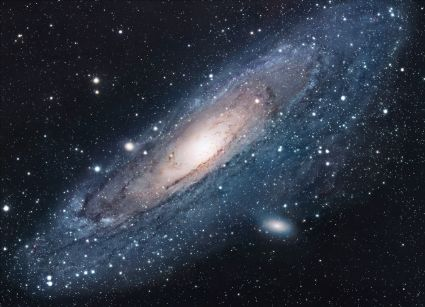
\includegraphics[scale=1.7]{imagenes/universe.jpg}
\caption{The Universe}
\label{fig:univerise}
\end{figure}

\subsubsection{Conclusion}
``una conclusion'' \citep{adams1995hitchhiker}

\bibliographystyle{plain}
\bibliography{references}
\end{document}
